\documentclass{article}
\usepackage[margin=2cm]{geometry}
\usepackage{float}
\usepackage{graphicx}

% Import custom listings colourings.
\usepackage{listings}
\usepackage{color}
\usepackage{xcolor}

%listings grey title/caption box 
\usepackage{caption}
\DeclareCaptionFont{white}{\color{white}}
\DeclareCaptionFormat{listing}{\colorbox{gray}{\parbox{\textwidth}{#1#2#3}}}
\captionsetup[lstlisting]{format=listing,labelfont=white,textfont=white}

% Java custom colours
\definecolor{javared}{rgb}{0.6,0,0} % for strings
\definecolor{javagreen}{rgb}{0.25,0.5,0.35} % comments
\definecolor{javapurple}{rgb}{0.5,0,0.35} % keywords
\definecolor{javadocblue}{rgb}{0.25,0.35,0.75} % javadoc

%Java custom config
\lstdefinestyle{customjava}{language=java,
basicstyle=\footnotesize,
keywordstyle=\color{javapurple}\bfseries,
stringstyle=\color{javared},
commentstyle=\color{javagreen},
morecomment=[s][\color{javadocblue}]{/**}{*/},
numbers=left,
numberstyle=\tiny\color{black},
stepnumber=1,
numbersep=10pt,
tabsize=4,
showspaces=false,
showstringspaces=false
}

%C++ custom colours
\definecolor{Brown}{cmyk}{0,0.81,1,0.60}
\definecolor{OliveGreen}{cmyk}{0.64,0,0.95,0.40}
\definecolor{CadetBlue}{cmyk}{0.62,0.57,0.23,0}

%C++ custom config
\lstdefinestyle{customcpp}{language=c++,
basicstyle=\footnotesize,
keywordstyle=\color{OliveGreen}\bfseries,
stringstyle=\color{javared},
commentstyle=\color{CadetBlue},
morecomment=[s][\color{javadocblue}]{/**}{*/},
numbers=left,
numberstyle=\tiny\color{black},
stepnumber=1,
numbersep=10pt,
tabsize=4,
showspaces=false,
showstringspaces=false}

\lstset{showspaces=false, showstringspaces=false,    basicstyle=\footnotesize, columns=fullflexible} 

% Paragraph settings
\setlength{\parskip}{10pt plus 1pt minus 1pt
\setlength{\parindent}{0cm}}

\begin{document}
\title{CS22510 - Assignment 1 \\ Runners and Riders - "Out and About"}
\author{Samuel Jackson \\ \texttt{slj11@aber.ac.uk}}
\date{\today}
\maketitle

\section{Event Creation Program Documentation}

\subsection{Code Listing}
The following section provides the full code listing for the event creation program. This application is written using C++. Doxygen documentation is available via the provided CD.

\lstinputlisting[style=customcpp, language=c++, caption={eventcreator.h}]{"../Event Creator/eventcreator.h"}
\lstinputlisting[style=customcpp, language=c++, caption={eventcreator.cpp}]{"../Event Creator/eventcreator.cpp"}

\lstinputlisting[style=customcpp, language=c++, caption={event.h}]{"../Event Creator/event.h"}
\lstinputlisting[style=customcpp, language=c++, caption={event.cpp}]{"../Event Creator/event.cpp"}

\lstinputlisting[style=customcpp, language=c++, caption={entrant.h}]{"../Event Creator/entrant.h"}
\lstinputlisting[style=customcpp, language=c++, caption={entrant.cpp}]{"../Event Creator/entrant.cpp"}

\lstinputlisting[style=customcpp, language=c++, caption={course.h}]{"../Event Creator/course.h"}
\lstinputlisting[style=customcpp, language=c++, caption={course.cpp}]{"../Event Creator/course.cpp"}

\lstinputlisting[style=customcpp, language=c++, caption={fileio.h}]{"../Event Creator/fileio.h"}
\lstinputlisting[style=customcpp, language=c++, caption={fileio.cpp}]{"../Event Creator/fileio.cpp"}

\lstinputlisting[style=customcpp, language=c++, caption={ioscanner.h}]{"../Event Creator/ioscanner.h"}
\lstinputlisting[style=customcpp, language=c++, caption={ioscanner.cpp}]{"../Event Creator/ioscanner.cpp"}


\subsection{Compilation Output}

\begin{center}
	\begin{lstlisting}[showstringspaces=false, caption={Build log of the C++ Event Creation Program}]
	
12:22:50 **** Build of configuration Debug for project Event Creator ****
make all 
Building file: ../course.cpp
Invoking: GCC C++ Compiler
g++ -O0 -g3 -Wall -c -fmessage-length=0 -MMD -MP -MF"course.d" -MT"course.d" -o "course.o" "../course.cpp"
Finished building: ../course.cpp
 
Building file: ../entrant.cpp
Invoking: GCC C++ Compiler
g++ -O0 -g3 -Wall -c -fmessage-length=0 -MMD -MP -MF"entrant.d" -MT"entrant.d" -o "entrant.o" "../entrant.cpp"
Finished building: ../entrant.cpp
 
Building file: ../event.cpp
Invoking: GCC C++ Compiler
g++ -O0 -g3 -Wall -c -fmessage-length=0 -MMD -MP -MF"event.d" -MT"event.d" -o "event.o" "../event.cpp"
Finished building: ../event.cpp
 
Building file: ../eventcreator.cpp
Invoking: GCC C++ Compiler
g++ -O0 -g3 -Wall -c -fmessage-length=0 -MMD -MP -MF"eventcreator.d" -MT"eventcreator.d" 
-o "eventcreator.o" "../eventcreator.cpp"
../eventcreator.cpp: In member function ‘int EventCreator::ChooseEvent()’:
../eventcreator.cpp:160:51: warning: comparison between signed and unsigned integer expressions [-Wsign-compare]
../eventcreator.cpp: In member function ‘char EventCreator::ChooseCourse(Event)’:
../eventcreator.cpp:194:52: warning: comparison between signed and unsigned integer expressions [-Wsign-compare]
Finished building: ../eventcreator.cpp
 
Building file: ../fileio.cpp
Invoking: GCC C++ Compiler
g++ -O0 -g3 -Wall -c -fmessage-length=0 -MMD -MP -MF"fileio.d" -MT"fileio.d" -o "fileio.o" "../fileio.cpp"
Finished building: ../fileio.cpp
 
Building file: ../ioscanner.cpp
Invoking: GCC C++ Compiler
g++ -O0 -g3 -Wall -c -fmessage-length=0 -MMD -MP -MF"ioscanner.d" -MT"ioscanner.d" -o "ioscanner.o" "../ioscanner.cpp"
../ioscanner.cpp: In member function ‘std::string IOScanner::ReadString(int)’:
../ioscanner.cpp:49:25: warning: comparison between signed and unsigned integer expressions [-Wsign-compare]
../ioscanner.cpp:52:29: warning: comparison between signed and unsigned integer expressions [-Wsign-compare]
Finished building: ../ioscanner.cpp
 
Building target: Event Creator
Invoking: GCC C++ Linker
g++  -o "Event Creator"  ./course.o ./entrant.o ./event.o ./eventcreator.o ./fileio.o ./ioscanner.o   
Finished building target: Event Creator
 

12:22:53 Build Finished (took 2s.319ms)
		
	\end{lstlisting}
\end{center}

\subsection{Session Output}

\begin{center}
	\begin{lstlisting}[showstringspaces=false, label={lst:create-output}, caption={Output of C++ Event Creation Program}]
----------------------
EVENT CREATION PROGRAM
----------------------

MAIN MENU
---------------------------
Enter an option: 
1 - Make new event
2 - Add entrants to event
3 - Create course for event
4 - Write an event to file
5 - View an event in the system
6 - Exit Program
1
Enter name of event:
MyNewEvent
Enter event date (DD/MM/YY):
16/3/13
Enter event start time (HH:MM):
12:00
Enter location of nodes file for event:
../event_3/nodes.txt
MAIN MENU
---------------------------
Enter an option: 
1 - Make new event
2 - Add entrants to event
3 - Create course for event
4 - Write an event to file
5 - View an event in the system
6 - Exit Program
3
Please choose an event:
0 - MyNewEvent
0
Enter nodes for course. Enter 0 to finish: 
1
3
4
9
12
14
1
0
MAIN MENU
---------------------------
Enter an option: 
1 - Make new event
2 - Add entrants to event
3 - Create course for event
4 - Write an event to file
5 - View an event in the system
6 - Exit Program
2
Please choose an event:
0 - MyNewEvent
0
Enter number of entrants to add: 
3
Enter entrant's name: 
Greg Jones
Please choose course for the entrant:
0 - A
0
Enter entrant's name: 
Bob Jones
Please choose course for the entrant:
0 - A
0
Enter entrant's name: 
Jane Doe
Please choose course for the entrant:
0 - A
0
MAIN MENU
---------------------------
Enter an option: 
1 - Make new event
2 - Add entrants to event
3 - Create course for event
4 - Write an event to file
5 - View an event in the system
6 - Exit Program
4
Please choose an event:
0 - MyNewEvent
0
MAIN MENU
---------------------------
Enter an option: 
1 - Make new event
2 - Add entrants to event
3 - Create course for event
4 - Write an event to file
5 - View an event in the system
6 - Exit Program
6
		
	\end{lstlisting}
\end{center}

\subsection{Generated Output Files}


\begin{center}
	\begin{lstlisting}[showstringspaces=false, caption={name.txt file output from listing \ref{lst:create-output}}]
	
MyNewEvent
16th March 2013
12:00

	\end{lstlisting}
\end{center}

\begin{center}
	\begin{lstlisting}[showstringspaces=false, caption={courses.txt file output from listing \ref{lst:create-output}}]

A 7 1 3 4 9 12 14 1 
		
	\end{lstlisting}
\end{center}

\begin{center}
	\begin{lstlisting}[showstringspaces=false, caption={entrants.txt file output from listing \ref{lst:create-output}}]

1 A Greg Jones
2 A Bob Jones
3 A Jane Doe	
		
	\end{lstlisting}
\end{center}

\section{Checkpoint Manager Program Documentation}

\subsection{Code Listing}
\lstinputlisting[style=customjava, language=java, caption={CheckpointManagerGUI.java}]{"../Checkpoint Manager/src/checkpoint/manager/gui/CheckpointManagerGUI.java"}

\lstinputlisting[style=customjava, language=java, caption={CheckpointManagerListener.java}]{"../Checkpoint Manager/src/checkpoint/manager/gui/CheckpointManagerListener.java"}

\lstinputlisting[style=customjava, language=java, caption={CheckpointManager.java}]{"../Checkpoint Manager/src/checkpoint/manager/datamodel/CheckpointManager.java"}

\lstinputlisting[style=customjava, language=java, caption={Entrant.java}]{"../Checkpoint Manager/src/checkpoint/manager/datamodel/Entrant.java"}

\lstinputlisting[style=customjava, language=java, caption={Course.java}]{"../Checkpoint Manager/src/checkpoint/manager/datamodel/Course.java"}

\lstinputlisting[style=customjava, language=java, caption={Checkpoint.java}]{"../Checkpoint Manager/src/checkpoint/manager/datamodel/Checkpoint.java"}

\lstinputlisting[style=customjava, language=java, caption={CPTimeData.java}]{"../Checkpoint Manager/src/checkpoint/manager/datamodel/CPTimeData.java"}

\lstinputlisting[style=customjava, language=java, caption={CPType.java}]{"../Checkpoint Manager/src/checkpoint/manager/datamodel/CPType.java"}

\lstinputlisting[style=customjava, language=java, caption={FileIO.java}]{"../Checkpoint Manager/src/checkpoint/manager/FileIO.java"}

\lstinputlisting[style=customjava, language=java, caption={ArgumentParseException.java}]{"../Checkpoint Manager/src/checkpoint/manager/exceptions/ArgumentParseException.java"}

\subsection{Compilation Output}

\subsection{Example Run}

\section{Event Manager Program Documentation}

\subsection{Compilation Output}
\begin{center}
	\begin{lstlisting}[showstringspaces=false, caption={Build log of the C Event Manager Program}]
	
12:27:50 **** Build of configuration Debug for project Event Manager ****
make all 
Building file: ../fileio.c
Invoking: GCC C Compiler
gcc -O0 -g3 -Wall -c -fmessage-length=0 -MMD -MP -MF"fileio.d" -MT"fileio.d" -o "fileio.o" "../fileio.c"
Finished building: ../fileio.c
 
Building file: ../linked_list.c
Invoking: GCC C Compiler
gcc -O0 -g3 -Wall -c -fmessage-length=0 -MMD -MP -MF"linked_list.d" -MT"linked_list.d" -o "linked_list.o" "../linked_list.c"
Finished building: ../linked_list.c
 
Building file: ../main.c
Invoking: GCC C Compiler
gcc -O0 -g3 -Wall -c -fmessage-length=0 -MMD -MP -MF"main.d" -MT"main.d" -o "main.o" "../main.c"
Finished building: ../main.c
 
Building file: ../util.c
Invoking: GCC C Compiler
gcc -O0 -g3 -Wall -c -fmessage-length=0 -MMD -MP -MF"util.d" -MT"util.d" -o "util.o" "../util.c"
Finished building: ../util.c
 
Building target: Event Manager
Invoking: GCC C Linker
gcc  -o "Event Manager"  ./fileio.o ./linked_list.o ./main.o ./util.o   
Finished building target: Event Manager
 

12:27:50 Build Finished (took 415ms)
		
	\end{lstlisting}
\end{center}
\subsection{Example Run Output}

\subsection{Example Run Results List}

\subsection{Output Of Log File}

\section{Outline of Programs}
This section of the document provides a brief outline of each of the three programs included as part of this project. This includes a discussion of the basic structure, design and operation of each application.

\subsection{Event Creation Program}
The event creation program is a command line based application written in C++. Its purpose is to create the event, courses and entrants file for each event. The design of the application allows the user to create multiple events at the same time, rather than having to make each event in serial. Because entrants need a course and a course needs an event, an event must be created before a course and a course must be created before an entrant. This includes the functionality to create different course and entrants associated with different events. Each event also expects a nodes file to be given when creating the event, allowing different events to work with different sets of allowed nodes. The user is also able to view an event by selecting the relevant option form the main menu.

Since lists of courses and entrants are associated with each event, I decided that the best approach would be to allow the user to create all the data about an event, then write it to file, rather than creating each of the files one at a time. When the user chooses the option to write an event, a new folder is created with the name of the event as the name of the folder. Inside the folder, the event, entrants and courses files are written.


\begin{figure}[H]
\centering
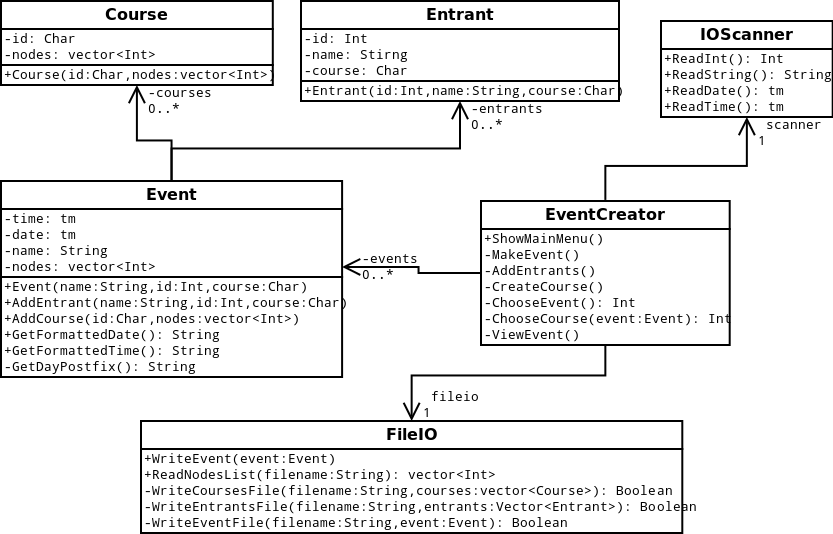
\includegraphics[width=0.6\textwidth]{diagrams/event_creator.png}
\caption{Class diagram of the Event Creator program. Getters/Setters not shown.}
\label{fig:GUI-image}
\end{figure}

\subsection{Checkpoint Manager Program}
The checkpoint manager program is written in Java and provides a Swing based GUI to allow the user to easily update entrants out in the field as the JVM allows the program to be executed on a variety of platforms. This program accepts the required files (entrants, courses, nodes, time and log files) as command line arguments using flags for each file. Help instructions are printed when no arguments or incorrect arguments are supplied. An example listing of arguments is supplied below:

\begin{center}
	\begin{lstlisting}[showstringspaces=false]
java -jar checkpoint_manager.jar -E ../../event_3/entrants.txt -C ../../event_3/courses.txt -K ../../event_3/nodes.txt
 -T ../../event_3/times.txt -L ../../event_3/log.txt

	\end{lstlisting}
\end{center}

The checkpoint manager program allows a race marshal to update the location of the entrants as they arrive at the various checkpoints on the course. Entrants are automatically excluded if checked into a checkpoint they should not of visited. The GUI also provides an option for marshals to excluded entrants based on failing a medical checkpoint. When an entrant is excluded, they are automatically removed from the list of available entrants. When an entrant is about to be excluded, the user is asked to confirm the operation, ensuring that they don't accidentally excluded a competitor.

\begin{figure}[H]
\centering
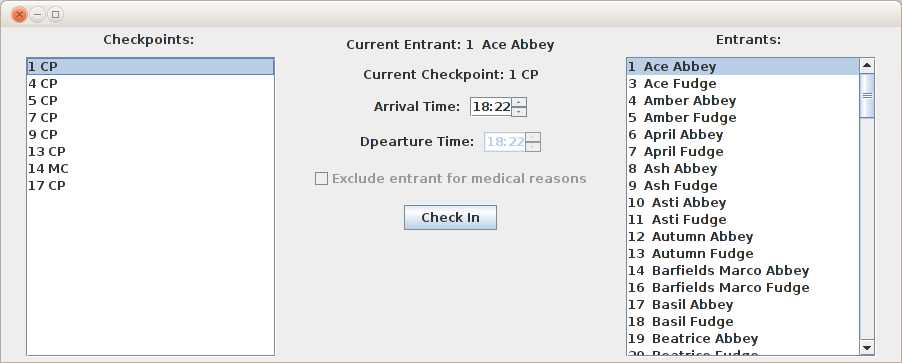
\includegraphics[width=0.5\textwidth]{img/GUI-screenshot.png}
\caption{Screen image of the Checkpoint manager GUI.}
\label{fig:GUI-image}
\end{figure}

\begin{figure}[H]
\centering
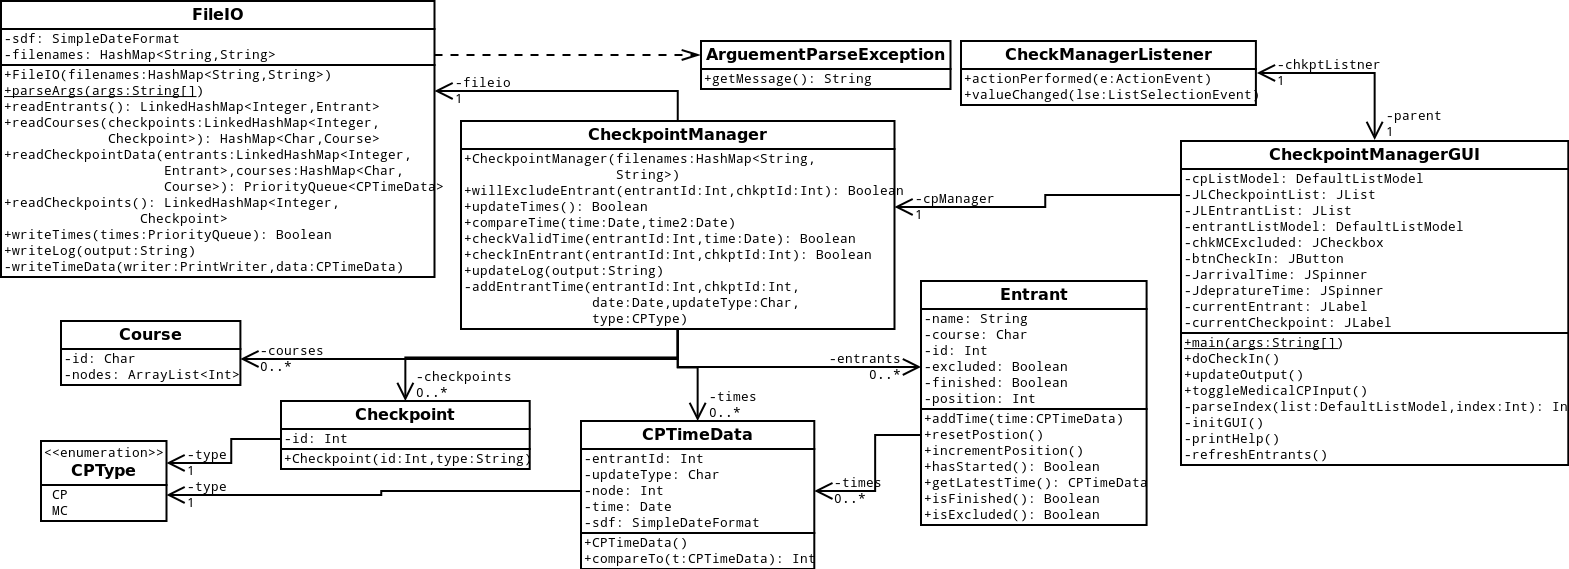
\includegraphics[width=1\textwidth]{diagrams/checkpoint_manager.png}
\caption{Class diagram of the Checkpoint Manager program. Getters/Setters not shown.}
\label{fig:GUI-image}
\end{figure}

The event manager program allows the user to input the time a competitor arrives and, in the case of medical checkpoints, departs. The program automatically checks that the arrival time is greater than the last time the entrant was checked in. In the case of medical checkpoints, it also checks that the arrival time is not greater than the departure time. Correct order of times is tracked using a priority queue.

\subsection{Event Manager Program}
The event manager program is written in C and handles checking the position and state of entrants as they progress through a course. This includes viewing a list of which entrants have been excluded, finished and are currently out on a track. It also gives the user the ability to query individual competitors and provides an estimate of what track/node they should/are on.

The event manager requires the loading of all the data files for an event. This is done by prompting the user at the start of the application and only needs to be done once. Like the event manager, the application locks the log and times file when reading to prevent multiple applications crashing during file processing.

\end{document}
